En las figuras \ref{fig:ej5-1}, \ref{fig:ej5-2} y \ref{fig:ej5-3}, vemos los gráficos obtenidos al simular el lote pedido en el enunciado para cada uno de los casos. Las tablas resumen las métricas solicitadas.

\begin{figure}[H]
  \centering
  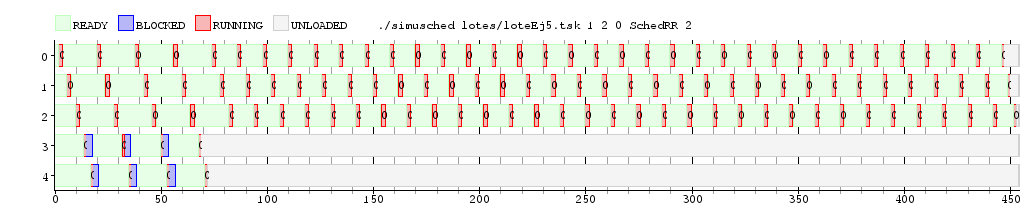
\includegraphics[width=1\textwidth]{img/imgEj5-1}
  \caption{}
  \label{fig:ej5-1}
\end{figure}

\begin{figure}[H]
  \centering
  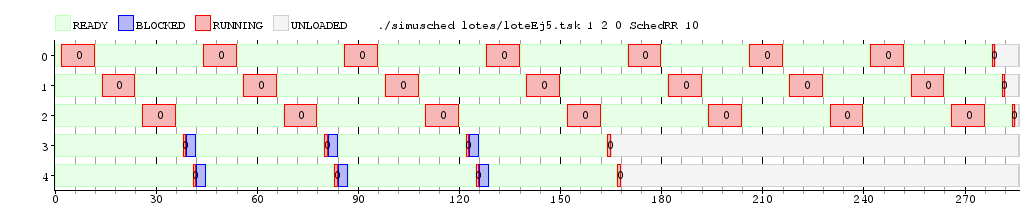
\includegraphics[width=1\textwidth]{img/imgEj5-2}
  \caption{}
  \label{fig:ej5-2}
\end{figure}

\begin{figure}[H]
  \centering
  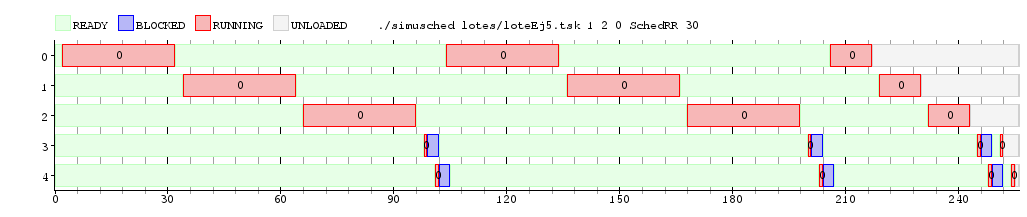
\includegraphics[width=1\textwidth]{img/imgEj5-3}
  \caption{}
  \label{fig:ej5-3}
\end{figure}

\begin{table}[H]
  \center
  \begin{center}
  \begin{tabular}{c|c|c|c|}
    \cline{2-4}
    & \multicolumn{3}{|c|}{\cellcolor{LightCyan}Latencia} \\
    \hline
    \rowcolor{LightCyan}
    \multicolumn{1}{|c|}{Quantum} & 2 & 10 & 30 \\
    \hline
    \multicolumn{1}{|c|}{\cellcolor{LightCyan}Tarea 0} & 2 & 2 & 2 \\
    \multicolumn{1}{|c|}{\cellcolor{LightCyan}Tarea 1} & 6 & 14 & 34 \\
    \multicolumn{1}{|c|}{\cellcolor{LightCyan}Tarea 2} & 10 & 26 & 66 \\
    \multicolumn{1}{|c|}{\cellcolor{LightCyan}Tarea 3} & 14 & 38 & 98 \\
    \multicolumn{1}{|c|}{\cellcolor{LightCyan}Tarea 4} & 17 & 41 & 100 \\
    \hline
    \multicolumn{1}{|c|}{\cellcolor{LightCyan}Promedio} & 9.8 & 24.2 & 60 \\
    \hline
  \end{tabular}
  \end{center}
  \caption{\footnotesize Latencia de cada tarea y latencia promedio según la duración del \emph{quantum} utilizado.}
  \label{tab:ej5-1}
\end{table}

\begin{table}[H]
  \center
  \begin{center}
  \begin{tabular}{c|c|c|c|}
    \cline{2-4}
    & \multicolumn{3}{|c|}{\cellcolor{LightCyan}\emph{Waiting time}} \\
    \hline
    \rowcolor{LightCyan}
    \multicolumn{1}{|c|}{Quantum} & 2 & 10 & 30 \\
    \hline
    \multicolumn{1}{|c|}{\cellcolor{LightCyan}Tarea 0} & 377 & 209 & 147 \\
    \multicolumn{1}{|c|}{\cellcolor{LightCyan}Tarea 1} & 380 & 212 & 160 \\
    \multicolumn{1}{|c|}{\cellcolor{LightCyan}Tarea 2} & 383 & 215 & 173 \\
    \multicolumn{1}{|c|}{\cellcolor{LightCyan}Tarea 3} & 60 & 156 & 243 \\
    \multicolumn{1}{|c|}{\cellcolor{LightCyan}Tarea 4} & 63 & 159 & 246 \\
    \hline
    \multicolumn{1}{|c|}{\cellcolor{LightCyan}Promedio} & 252.6 & 190.2 & 193.8 \\
    \hline
  \end{tabular}
  \end{center}
  \caption{\footnotesize Tiempo total de espera de cada tarea y promedio según la duración del \emph{quantum} utilizado.}
  \label{tab:ej5-2}
\end{table}

\begin{table}[H]
  \center
  \begin{center}
  \begin{tabular}{c|c|c|c|}
    \cline{2-4}
    & \multicolumn{3}{|c|}{\cellcolor{LightCyan}\emph{Turn-around}} \\
    \hline
    \rowcolor{LightCyan}
    \multicolumn{1}{|c|}{Quantum} & 2 & 10 & 30 \\
    \hline
    \multicolumn{1}{|c|}{\cellcolor{LightCyan}Tarea 0} & 447 & 279 & 217 \\
    \multicolumn{1}{|c|}{\cellcolor{LightCyan}Tarea 1} & 450 & 282 & 230 \\
    \multicolumn{1}{|c|}{\cellcolor{LightCyan}Tarea 2} & 453 & 285 & 243 \\
    \multicolumn{1}{|c|}{\cellcolor{LightCyan}Tarea 3} & 69 & 165 & 252 \\
    \multicolumn{1}{|c|}{\cellcolor{LightCyan}Tarea 4} & 72 & 168 & 255 \\
    \hline
    \multicolumn{1}{|c|}{\cellcolor{LightCyan}Promedio} & 298.2 & 235.8 & 239.4 \\
    \hline
  \end{tabular}
  \end{center}
  \caption{\footnotesize Tiempo total de ejecución de cada tarea (\emph{turn-around}) y promedio según la duración del \emph{quantum} utilizado.}
  \label{tab:ej5-3}
\end{table}


Se puede notar que, a la hora de optimizar la latencia, el \emph{quantum} que mejor lo hace es el de 2 ciclos, y a medida que aumenta empeora la métrica. Esto es totalmente razonable puesto que los procesos que están en la cola de espera tienen que esperar (valga la redundancia) a que los procesos que ejecutan antes completen sus \emph{quantums} (o bien se bloqueen o terminen). Al tener un \emph{quantum} pequeño, la espera de cada proceso para empezar a ejecutar también lo es.

En contraposición, el \emph{quantum} de menor tamaño tiene un pobre desempeño a la hora de considerar el \emph{waiting time} o el \emph{turn-around}. \footnote{Notar que el segundo es consecuencia directa del primero, pues el tiempo total es la suma del tiempo efectivamente utilizado en la CPU más el tiempo de espera. Entonces nos centraremos principalmente en el \emph{waiting-time}.} En efecto, si notamos que la duración del \emph{quantum} es igual a la duración del cambio de contexto, no resulta sorprendente ver estos resultados: cerca de la mitad del tiempo total que se requiere para que el lote completo termine de procesar se gasta haciendo \emph{contex-switch}. Para ser más exactos, en total se pasan 221 ciclos de reloj procesando tareas\footnote{Tres tareas usan el CPU 70 ciclos, y las otras dos usan 3 ciclos para hacer tres llamadas de \emph{I/O}. Además, hay que considerar que cada tarea gasta un ciclo extra para terminar. Eso nos da $70\times 3 + 3 + 3\times 2 + 2 = 221$} y 232 haciendo cambios de contexto. Esto repercute fuertemente en el tiempo de espera de las tareas.

Para \emph{quantums} de tamaño 10 y 30, el \emph{waiting-time} resulta sigificativamente menor. Aunque, como puede verse en la tabla \ref{tab:ej5-2}, el tiempo de espera promedio no varía demasiado entre ambos casos, un análisis más detallado nos permite ver que la composición de dichos promedios si que es distinta. Si consideramos las tareas 0, 1 y 2 (que son las que solo consumen CPU en gran cantidad) vemos que su tiempo de espera se reduce notablemente al incrementar el \emph{quantum} de 10 a 30. Sin embargo, en contraste las tareas 3 y 4 (que apenas usan el CPU para realizar llamadas de \emph{I/O}) ven incrementados sus tiempos de espera en forma aún más significativa. Esto se explica porque mientras que por un lado el aumento del \emph{quantum} no beneficia a las tareas bloqueantes (pues las mismas solo requieren un ciclo), sí lo hace para las tareas de alto consumo de CPU. Pero este beneficio perjudica indirectamente al \emph{waiting-time} del resto de las tareas, incluso al de otros procesos de CPU, aunque en este caso queda absorbido por el propio beneficio.

De hecho, los procesos bloqueantes muestran su menor tiempo de espera cuando el \emph{quantum} es de 2 ciclos. Sin embargo, como ya vimos el dimensionamiento del \emph{quantum} respecto del cambio de contexto es tan malo que en términos generales no tiene sentido considerar esta opción, y aún en caso de estar en una situación donde atender \emph{I/O} rápido sea prioritario, es preferible explorar otras alternativas de \emph{scheduling} que aprovechen mejor el procesador (como \emph{multilevel feedback-queue scheduling}). Entre los \emph{quantums} de 10 y 30 ciclos puede preferirse uno u otro según la importancia relativa que se le asigne a atender rápido procesos bloqueantes y terminar pronto con procesos largos.